\def\hnumber{3}
\def\student{Jerry Sun}
\def\studentid{ys7va}
\documentclass{cs4444}
\usepackage{tikz, pgfplots, graphicx}
\begin{document}

\maketitle

\section{Problem Description}
The goal of this assignment is to write a parallel C program using openmpi to optimize the runtime for a lightly twisted classic heated plate problem, and to discover the performance regarding several concerns around parallel program like overhead, efficiency, etc. 

The halo problem I am dealing with here has the setting as below:
	\begin{itemize}
	\item The interior cells should all initialized to the same temperature (50 degrees)
	\item The border cells fixed at a specific temperature (0 degrees along the top and left sides and 100 degrees along the bottom and right sides)
	\item There is a single internal condition (col=6500 \& row=4500) in which a single cell is held at 1000 degrees
	\item  In each time step of the simulation, the temperature of each cell is computed by averaging the temperatures of the four neighboring cells in the previous time step
	\end{itemize}
	
The original sequential program provided has a runtime of 1671 seconds for a 10000 iterations on $10000 * 10000$ plates

\section{Result Summary}
For 10000 iterations on $10000 * 10000$ plates with the hotspot, my final parallel program works, and gives the best performance with 2 ghost cell layers which takes 27 seconds to finish including the final image rendering. The overall speedup is 67 times faster than the original sequential program.

\section{Metadata}
\subsection{Software}
	SLURM: version 14.11
	
	GNU bash: version 4.1.2
	
	openmpi: version 1.8.4
	
	gcc: version 4.4.7

\subsection{Hardware}
	10 core Intel(R) Xeon(R) CPU E5-2670 v2 @ 2.50GHz with a cache size of 25600KB
	
\section{Approach}
	For this assignment, it is required to parallelize the particular halo problem described above. There are several main core designs I use to implement the parallelized version of halo.
	\subsection{Divide \& Ghost Cell}
		For a given number of nodes and a fixed size plate, I want to divide the   
			whole plate evenly onto each node, so that it can distribut the computation evenly across different nodes. Here, in particular I divide the whole plate in a row-major order, as each node will be responsible for a number of continuous rows with 
				all columns. The reason and the advantage of this approach can be found in Optimization section later.
				
		However, if each node only maintain the cells that it needs to compute, the result will not be accurate, since the outer cells might need the information from neighbor nodes to maintain their accuracy. Therefore, I add the ghost cells around the core block. These ghost cells will receive the value of the corresponding cells in the neighboring nodes, thus providing the center block values to compute with. 
		
		Unfortunately, the other problem is that the ghost cells will still loose its accuracy since they are now on the boundary. Therefore, the program need to routinely update the ghost cells, and the thickness of the ghost cells directly determines how often do does it need to do the update(detail see next subsection).
		
		\subsection{Message Passing}
		Message passing is extremely tricky to deal with in parallel program. We want to maintain the accuracy, while achieving a higher efficiency(also avoiding deadlocks) since the overhead of message passing between nodes will deprecate the performance of the whole program especially when there is a large number of nodes, like 200.

			The approach here I need to consider includes two parts, first is how often does the program need to send the message, next is how is it going to send values.

			First, for a fixed thickness of the ghost cell, say n cells thick, the program can maintain its accuracy in the "core blocks" for n iterations, since for each iteration, one single row of cells, from edge to the center, will lose its accuracy. Therefore it only need to transfer the value of cells every n iterations instead of every single iterations. 
			
			Second, the most important aspect regarding message passing is the way to implement the send/receive patterns since it is extremely easy to have deadlock or really inefficient sending pattern. Our design classify all message transfer into four categories as follow:
	\begin{itemize}			
	\item tag 0: even node to odd node upward send
	\item tag 1: odd to even upward send
	\item tag 2: even to odd downward send
	\item tag 3: odd to even downward send
	\end{itemize}
	Note: upward send just means from lower rank node to higher rank node, and downward send just means the opposite way.
	
	Then for a single odd-rank node, it will perform the following 4 steps:
				\begin{itemize}			
	\item receive ghost cells from lower even node
	\item send ghost cells to higher even node 
	\item receive ghost cells from higher even node
	\item send ghost cells to lower even node
		\end{itemize}
	
	For a even-rank node then it just perform the other way around.
	
	Note that during implementation, it also needs to separate the first and last node, since they only need to do one send and one receive. For node 0 it is simple, since it only need to handle tag 0 and tag 3. However, for the last node, there are actually two cases. If the number of nodes is even, then the last node has odd rank. Therefore it needs to handle tag 0 and tag 3. However, if the number of nodes is odd, then it needs to handle the other two tags. 
	
	After all those steps, our message transfer can be grouped into 4 tags and inside each tag, all message passing can happen simultaneously, thus providing better performance.
	
\section{Performance}
	In this section, I will give a brief analysis for the data I retrieved from the testing above. For time measurement, I use the \textit{time()} function in `time.h` library. For timing, it counts the total runtime from the start of the program, to the point right after \textit{MPI\_Finalize()}.
	 
	Since the clock time of the program running on Rivanna varies, I retrieve the optimal runtime for each condition. Also, the process to create snapshot is related to file write which takes extra time to finish, so for all experiments the program only produces one final snapshot after 10000 iterations.

\subsection{Runtime data collection}
	Followed are all the timing recorded during testing on Rivanna based on different number of tasks, number of iterations per cell and different number of ghost cells.
	
\begin{center}
\begin{table}[ht]
\caption{200 tasks}
\centering
\begin{tabular}{c c c c}
\hline\hline
iter per cell & 1 ghost layer & 2 ghost layer & 3 ghost layer \\
\hline
1&30&27	&28 \\
2&50&52	&56 \\
4&79&82	&88 \\
\hline
\end{tabular}
\caption{100 tasks}
\centering
\begin{tabular}{c c c c}
\hline\hline
iter per cell & 1 ghost layer & 2 ghost layer & 4 ghost layer \\
\hline
1&56&57&60 \\
2&97&99&103\\
4&157&159&165\\
\hline
\end{tabular}
\caption{20 tasks}
\centering
\begin{tabular}{c c c c}
\hline\hline
iter per cell & 1 ghost layer & 2 ghost layer & 4 ghost layer \\
\hline 
1&266&263&266 \\
2&474&473&477 \\
4&773&774&779 \\
\hline
\end{tabular}
\end{table}
\end{center}

\subsection{Ghost Cell Analysis}
First, I want to explore the runtime differences between different number of ghost cells. The following graph shows the runtime comparison regarding different number of ghost cells with 200 tasks.
\begin{center}
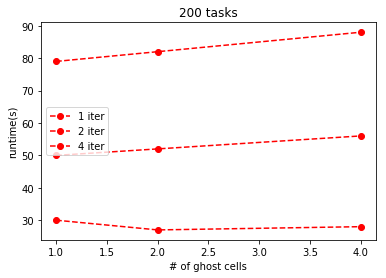
\includegraphics[width=8cm, height=6cm]{fix_nodes}
\end{center}
From the graph above we can see that there is no significant difference regarding the performance of different number of ghost cells. This is mainly due to the fact that while a larger number of ghost cells can lead to a smaller number of message passing, the total amount of the data that need to be transferred increases, also to maintain the accuracy of the center blocks the program also need to have more calculations for each node within the extra ghost cells. Both of those two aspects might cancel out the advantage of fewer message passing.

\subsection{Granularity Analysis}
Second, I want to explore the effect of increasing granularity. If the program only increases the number of computations while maintain any other aspects (simply by executing the "averaging process" multiple times), how will the performance be affected? Here I pick all the results for 1 single ghost cell.
 
\begin{center}
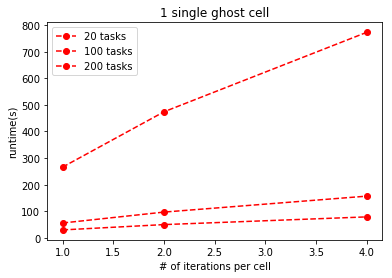
\includegraphics[width=8cm, height=6cm]{fix_ghost}
\end{center}

We can find that the growth in runtime is not proportional to  the growth in the number of iterations per cell. This is simply because of the overhead due to the message passing. Especially when 200 tasks are deployed, if there is no overhead, the theoretical runtime for 4 iterations per cycle should be $4 * 30 = 120$, but in reality the run time is only $80$. This means that a large proportion of the runtime for 1 iteration per cell is caused by overhead, including initiating MPI, message passing, etc.

\subsection{Tasks Analysis}

Finally, I want to explore the influence of deploying more tasks and the corresponding efficiency score. Here I pick all the results for 1 ghost cell.

\begin{center}
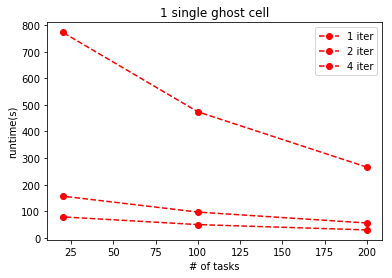
\includegraphics[width=8cm, height=6cm]{task_vs_time}
\end{center}

From the graph on the left, we can see non-trivial improvement in performance given an increasing number of tasks. While there exists overhead observed at prior sections, I can still state that the performance gain at 200 tasks level is significant.

\section{Optimization} 

\subsection{row-major division}
Here I prefer to divide the plate into multiple rows with different columns instead of a usual column division technique shown in class/textbook. The main criteria I want to consider for memory alignments are cache locality during computation and the message passing expense. For the cache locality, inside the for loop we typically choose to have the outer loop as rows and the inner loop as columns. Therefore a row-major division can give a decent cache performance by accessing continuous memory. The other advantage row-major division has is that when sending cells' value to other nodes, the program always wants to send continuous memory. Therefore, a row-major data division will be corresponding to the way cell values are stored in the initial/final maps. 

\subsection{message passing}
As discussed earlier in Approach, the message passing design is an extremely important optimization compared to a regular linear send/receive process. For one single processor, the theoretical lower bound for message-passing function it has to call is 4 (two sends and two receives). Our current implementation actually meets this lower bound, as each processor will finish its message passing task without extra wait time because of the design problem. 

 Also, I have tested asynchronous message passing using ISEND, IRECEIVE in a smaller scale. However, the result shows that there is no significant performance bonus using those two methods compared to the performance using SEND/RECEIVE.
 
\section{conclusion}
In this assignment, I have gain solid experience in designing and implementing parallel program using MPI. The parallel program I implemented shows a substantial performance speedup than the original sequential program with a speedup rate over $60$ times. Also, the observation made within different circumstances indicates the influence of overhead created by message passing is significant especially in large number of tasks. At the same time, however, simply reducing rate of the message passing by increasing number of ghost cell layers doesn't have a solid improvement for the overall performance because of other disadvantages using this technique.  
\section{Pledge}

\pledge
\newpage
\section{Appendix}
\subsection{halo.c}
\lstinputlisting[language=c]{halo.c}
\newpage
\subsection{halo.slurm}
\lstinputlisting[language=bash]{halo.slurm}





\end{document}
